\documentclass[12pt]{article}
\usepackage{note}

\title{Vector boson decay opening angle}
\author{Ivan Pogrebnyak}
\date{\today}

\begin{document}
\maketitle

\begin{figure}[H]
  \centering
  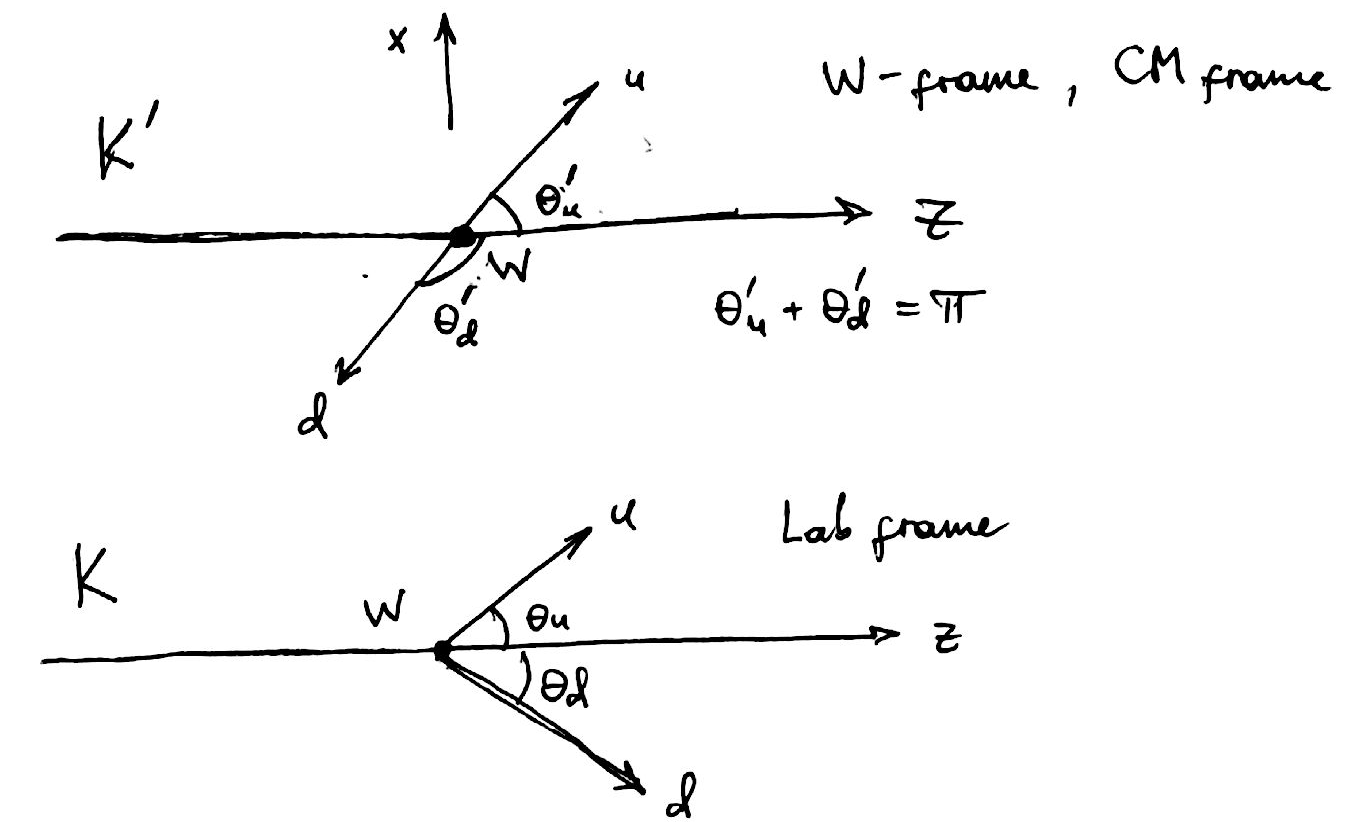
\includegraphics[width=0.65\textwidth]{fig/fig.png}
\end{figure}

{\bf In the lab frame, $K$:}
\begin{equation}
  P_W = (E_W,0,0,p_W), \quad
  P_u = (E_u,p_u\sin\theta_u,0,p_u\cos\theta_u), \quad
  P_d = (E_d,-p_d\sin\theta_d,0,p_d\cos\theta_d)
\end{equation}
%
Since $m_u\ll E_u$ and $m_d\ll E_d$,
\begin{equation}
  P_u = (E_u,E_u\sin\theta_u,0,E_u\cos\theta_u), \quad
  P_d = (E_d,-E_d\sin\theta_d,0,E_d\cos\theta_d)
\end{equation}
%
By conservation of momentum,
\begin{equation}\label{eq:cons}
  \left\{\begin{array}{l}
    E_W = E_u + E_d, \\
    E_u\sin\theta_u = E_d\sin\theta_d, \\
    p_W = E_u\cos\theta_u + E_d\cos\theta_d.
  \end{array}\right.
  \quad
  \begin{array}{l}
    +\begin{array}{l}
      E_d^2\cos^2\theta_d = p_W^2 + E_u^2\cos^2\theta_u - 2p_WE_u\cos\theta_u \\
      E_u^2\sin^2\theta_u = E_d^2\sin^2\theta_d
    \end{array} \\
    \hline
    \hspace{17mm} E_d^2 = p_W^2 + E_u^2 - 2p_WE_u\cos\theta_u
  \end{array}
\end{equation}
%
\begin{equation}\label{eq:cos}
  \therefore
  \cos\theta_u = \frac{p_W^2 + E_u^2 - E_d^2}{2p_WE_u}
\end{equation}
%
\begin{equation}\label{eq:pW}
  E^2 = p^2 + m^2 \quad \Rightarrow \quad
  p_W = \sqrt{E_W^2-m_W^2} = E_W\sqrt{1 - \left(\frac{m_W}{E_W}\right)^2}
%  \approx E_W\left( 1 - \frac{1}{2}\left(\frac{m_W}{E_W}\right)^2 \right)
\end{equation}

%%%%%%%%%%%%%%%%%%%%%%%%%%%%%%%%%%%%%%%%%%%%%%%%%%%%%%%%%%%%%%%%%%%%%%%%%%

{\bf In the CM frame, $K'$:}
\begin{equation}\label{eq:pCM}
  P'_W = (m_W,0,0,0), \quad
  P'_u = (E'_u,p'_u\sin\theta'_u,0,p'_u\cos\theta'_u), \quad
  P'_d = (E'_d,-p'_d\sin\theta'_d,0,p'_d\cos\theta'_d).
\end{equation}
\begin{equation}\label{eq:pud}
  P'_u = (E'_u,E'_u\sin\theta'_u,0,E'_u\cos\theta'_u), \quad
  P'_d = (E'_d,-E'_d\sin\theta'_d,0,E'_d\cos\theta'_d).
\end{equation}
%
There is no net momentum in the CM frame, so from \eq{pud} and \ref{eq:pCM},
\begin{equation}
  E'_u = E'_d = \frac{m_W}{2}, \quad \text{and} \quad
  \theta'_u + \theta'_d = \pi
\end{equation}
\begin{equation}
  \sin\theta'_u = \sin\theta'_d, \quad \text{and} \quad
  \cos\theta'_u = -\cos\theta'_d
\end{equation}
%
So,
\begin{equation}\label{eq:pud2}
  P'_u = \frac{m_W}{2}(1, \sin\theta'_u,0, \cos\theta'_u), \quad
  P'_d = \frac{m_W}{2}(1,-\sin\theta'_u,0,-\cos\theta'_u).
\end{equation}

%%%%%%%%%%%%%%%%%%%%%%%%%%%%%%%%%%%%%%%%%%%%%%%%%%%%%%%%%%%%%%%%%%%%%%%%%%
\pagebreak

{\bf Special case, $\theta'_u=\pi/2$:}\\
%
By symmetry,
\begin{equation}
  E_u = E_d = \frac{E_W}{2}% = \frac{\gamma m_w}{2}
\end{equation}
%
Substituting into \eq{cos},
\begin{equation}
  \cos\theta_u = \frac{p_W^2 + E_u^2 - E_d^2}{2p_WE_u}
  = \frac{p_W}{2E_u} = \frac{p_W}{E_W}
\end{equation}
\begin{equation}
  \sin\theta_u = \sqrt{1 - \cos^2\theta_u}
  = \sqrt{1 - \frac{p_W^2}{E_W^2}}
\end{equation}
%
Applying \eq{pW},
\begin{equation}
  \sin\theta_u = \sqrt{1 - \left(1 - \left(\frac{m_W}{E_W}\right)^2\right)}
  = \frac{m_W}{E_W}
\end{equation}
%
For high energy $W$, the angle between the transversely emitted quarks in the lab frame can be approximated as
\begin{equation}\label{eq:theta}
  \boxed{
    \theta = 2\theta_u \approx 2\sin\theta_u = \frac{2m_W}{E_W}
  }
\end{equation}
This is in fact asymptotically minimum angle.

%%%%%%%%%%%%%%%%%%%%%%%%%%%%%%%%%%%%%%%%%%%%%%%%%%%%%%%%%%%%%%%%%%%%%%%%%%

{\bf General case:}
%
\begin{equation}
  P_W = \Lambda P'_W \quad \Leftrightarrow \quad
%
  \begin{pmatrix} E_W\\0\\0\\p_W \end{pmatrix} =
  \begin{pmatrix}
    \gamma & 0 & 0 & \gamma\beta \\
    0 & 1 & 0 & 0 \\
    0 & 0 & 1 & 0 \\
    \gamma\beta & 0 & 0 & \gamma \\
  \end{pmatrix}
  \begin{pmatrix} m_W\\0\\0\\0 \end{pmatrix}
  \quad \Rightarrow \quad
%
  \left\{\begin{array}{l}
    E_W = \gamma m_W \\
    p_W = \gamma\beta m_W
  \end{array}\right.
\end{equation}
\begin{equation}
  \gamma = \frac{E_W}{m_W}, \quad
  \gamma\beta = \frac{p_W}{m_W}, \quad
  \beta = \frac{p_W}{E_W}
\end{equation}
%
\begin{equation}
  E_q \begin{pmatrix}
    1 \\
    \pm\sin\theta_q \\
    0 \\
    \cos\theta_q
  \end{pmatrix} =
  P_q = \Lambda P'_q =
  \frac{m_W}{2}
  \begin{pmatrix}
    \gamma & 0 & 0 & \gamma\beta \\
    0 & 1 & 0 & 0 \\
    0 & 0 & 1 & 0 \\
    \gamma\beta & 0 & 0 & \gamma \\
  \end{pmatrix}
  \begin{pmatrix} 1\\ \pm\sin\theta'_u\\ 0\\ \pm\cos\theta'_u \end{pmatrix}
  = \frac{m_W}{2}
  \begin{pmatrix}
    \gamma \pm \gamma\beta\cos\theta'_u \\
    \pm\sin\theta'_u \\
    0 \\
    \gamma\beta \pm \gamma\cos\theta'_u
  \end{pmatrix}
\end{equation}
%
\begin{equation}
  E_q = \frac{m_W}{2} (\gamma \pm \gamma\beta\cos\theta'_u)
  = \frac{E_W}{2} (1 \pm \beta\cos\theta'_u)
\end{equation}
%
Substituting into \eq{cos},
\begin{align}
  \cos\theta_u &= \frac{p_W^2 + E_u^2 - E_d^2}{2p_WE_u}
  = \frac{\beta^2 E_W^2 + \frac{E^2_W}{4}\left[(1 + \beta\cos\theta'_u)^2 - (1 - \beta\cos\theta'_u)^2\right]}{\beta E_W^2(1 + \beta\cos\theta'_u)}
  \nonumber \\
  &= \frac{\beta^2 + \frac{1}{4}\left[(1 + \beta\cos\theta'_u)^2 - (1 - \beta\cos\theta'_u)^2\right]}{\beta (1 + \beta\cos\theta'_u)}
  = \frac{\beta^2 + \beta\cos\theta'_u}{\beta (1 + \beta\cos\theta'_u)}
  = \frac{\beta + \cos\theta'_u}{1 + \beta\cos\theta'_u}
\end{align}
Likewise,
\begin{align}
  \cos\theta_d &= \frac{p_W^2 + E_d^2 - E_u^2}{2p_WE_d}
  = \frac{\beta^2 E_W^2 + \frac{E^2_W}{4}\left[(1 - \beta\cos\theta'_u)^2 - (1 + \beta\cos\theta'_u)^2\right]}{\beta E_W^2(1 - \beta\cos\theta'_u)}
  = \frac{\beta - \cos\theta'_u}{1 - \beta\cos\theta'_u}
\end{align}
%
\begin{equation}
  \sin\theta_q = \sqrt{1 - \cos^2\theta_q}
  = \sqrt{1 - \left(\frac{\beta \pm \cos\theta'_u}{1 \pm \beta\cos\theta'_u}\right)^2}
  = \frac{\sin\theta'_u}{\gamma \pm \gamma\beta\cos\theta'_u}
\end{equation}
%
\begin{equation}
  \gamma = \frac{E_W}{m_W}, \quad
  \beta = \frac{p_W}{E_W} = \frac{\sqrt{E_W^2-m_W^2}}{E_W}
  = \sqrt{1-\left(\frac{m_W}{E_W}\right)^2}
  = \sqrt{1-\gamma^{-2}}
\end{equation}
\begin{equation}
  \gamma\beta = \frac{p_W}{m_W} = \frac{\sqrt{E_W^2-m_W^2}}{m_W}
  = \sqrt{\left(\frac{E_W}{m_W}\right)^2 - 1}
  = \sqrt{\gamma^2 - 1}
\end{equation}
%
\begin{equation}\label{eq:sin}
  \boxed{
    \sin\theta_q
    = \frac{\sin\theta'_u}{\gamma \pm \sqrt{\gamma^2 - 1}\cos\theta'_u}
  }
\end{equation}
This is the exact result.
Only the approximation of massless quarks has been made, which is very accurate, given the mass of $W$ is $m^W=80.4\GeV$ and the masses of the quarks are $m^u=2.3\MeV$ and $m^d=4.8\MeV$.
\vspace{5mm}

In the limit of large $\gamma$,
\begin{equation}
  \sin\theta_q
  = \frac{\sin\theta'_u}{\gamma (1\pm\cos\theta'_u)}
  \approx \theta_q
\end{equation}
%
The angle between emitted quarks is then
\begin{equation}
  \theta \approx \frac{\sin\theta'_u}{\gamma (1 + \cos\theta'_u)}
               + \frac{\sin\theta'_u}{\gamma (1 - \cos\theta'_u)}
  = \frac{2}{\gamma}\frac{1}{\sin\theta'_u}
\end{equation}
This gives \eq{theta}, for $\theta'_u=\pi/2$.
%\eq{theta} cannot be recovered directly from \eq{sin} as for a small
%$\gamma$ the opening angle is not small.

%Calculating the sum of sines directly from \eq{sin},
%
%\begin{align}
%  \sin\theta_u + \sin\theta_d
%  &= \frac{\sin\theta'_u}{\gamma + \sqrt{\gamma^2 - 1}\cos\theta'_u}
%   + \frac{\sin\theta'_u}{\gamma - \sqrt{\gamma^2 - 1}\cos\theta'_u}
%  \nonumber \\
%  &= \frac{\sin\theta'_u(\gamma + \sqrt{\gamma^2 - 1}\cos\theta'_u + \gamma - \sqrt{\gamma^2 - 1}\cos\theta'_u)}{\gamma^2 - (\gamma^2 - 1)\cos^2\theta'_u}
%  \nonumber \\
%  &= \frac{2\gamma\sin\theta'_u}{1+(\gamma^2-1)\sin^2\theta'_u}
%\end{align}

\vspace{5mm}
\eq{sin} can be expressed as a tangent. Let $\sin\theta = A/B$, then
\begin{equation}
  \tan\theta = \frac{\sin\theta}{\cos\theta}
  = \frac{\sin\theta}{\sqrt{1-\sin^2\theta}}
  = \frac{A/B}{\sqrt{1-A^2/B^2}}
  = \frac{A}{\sqrt{B^2-A^2}}
\end{equation}
%
From \eq{sin},
\begin{align}
  B^2-A^2 &= \gamma^2 + (\gamma^2-1)\cos^2\theta'_u \pm 2\gamma\sqrt{\gamma^2-1}\cos\theta'_u - \sin^2\theta'_u
  \nonumber \\
  &= \gamma^2 + \gamma^2\cos^2\theta'_u \pm 2\gamma\sqrt{\gamma^2-1}\cos\theta'_u - 1
  \nonumber \\
  &= (\gamma^2-1) \pm 2\gamma\sqrt{\gamma^2-1}\cos\theta'_u + \gamma^2\cos^2\theta'_u
  \nonumber \\
  &= \left( \sqrt{\gamma^2-1} \pm \gamma\cos\theta'_u \right)^2
   = \gamma^2 \left( \beta \pm \cos\theta'_u \right)^2.
\end{align}
Therefore,
\begin{equation}\label{eq:tan}
  \boxed{
    \tan\theta_q
    = \frac{\sin\theta'_u}{\gamma\left( \beta \pm \cos\theta'_u \right)}
  }
\end{equation}
%
Using the tangen of sum equation,
\begin{equation}
  \tan\theta_\mathrm{opening} = \tan(\theta_u+\theta_d)
  = \frac{\tan\theta_u+\tan\theta_d}{1-\tan\theta_u\tan\theta_d}
  = \frac{2\beta\gamma\sin\theta'_u}{(\gamma^2-1)\sin^2\theta'_u - 1}
  = \frac{2(\beta\gamma\sin\theta'_u)}{(\beta\gamma\sin\theta'_u)^2 - 1}
\end{equation}

\begin{equation}\label{eq:result}
  \boxed{
    \theta_\mathrm{opening}
    = \tan^{-1}\left[
      \frac{2(\beta\gamma\sin\theta'_u)}{(\beta\gamma\sin\theta'_u)^2 - 1}
    \right]
  }
\end{equation}

\begin{figure}[H]
  \centering
  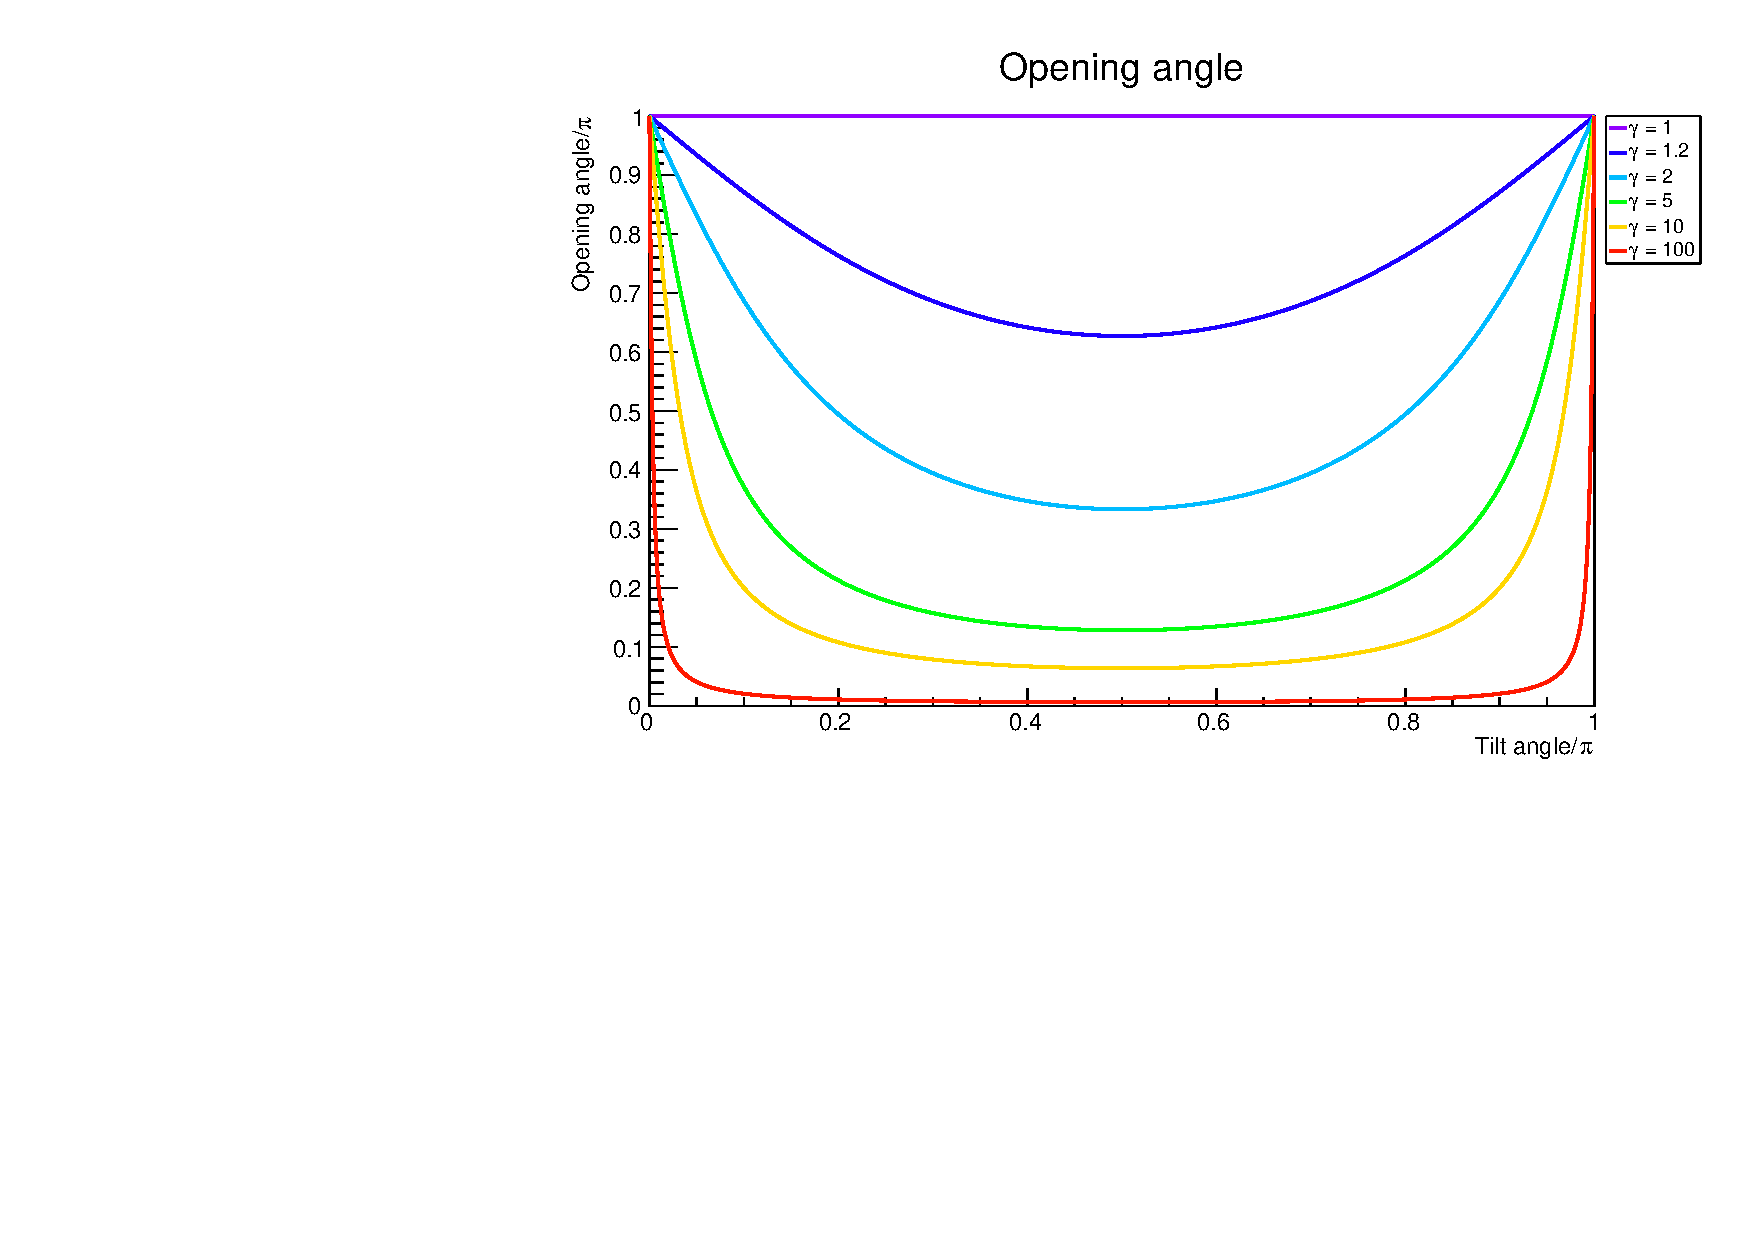
\includegraphics[width=\textwidth]{fig/opening_angle.pdf}
\end{figure}

\end{document}
